%\documentclass[handout,ignorenonframetext,red]{beamer}
\documentclass[ignorenonframetext,red]{beamer}
%\documentclass[class=article, a4paper]{beamer}
%\documentclass[handout]{beamer} %pour sortie papier


\usepackage[french]{babel}
\usepackage{pgf,pgfarrows,pgfn odes,pgfautomata,pgfheaps,pgfs hade}
\usepackage{amsmath,amssymb}
\usepackage[utf8]{inputenc}
\usepackage{stmaryrd}
\usepackage{url}


%\documentclass[svgnames,ignorenonframetext]{beamer}
%\usepackage{times}
\usepackage{listings}
\usepackage{amsmath,multicol}
\usepackage{verbatim}
%\usepackage{beamerarticle}
\usepackage{longtable}
%\usepackage{ucs}
%\usepackage[utf8]{inputenc}
\usepackage{pdfpages}

\setcounter{tocdepth}{1}

\mode<presentation>
{
  \usetheme{Warsaw}
  \setbeamercovered{transparent}
  \AtBeginSection[]
  {
    \begin{frame}<beamer>
       \setcounter{tocdepth}{2}
       \tableofcontents[currentsection,currentsubsection,hideothersubsections]
    \end{frame}
  }

  \AtBeginSubsection[]
  {
    \begin{frame}<beamer>
    \frametitle{\thesection. \insertsectionhead}
       \tableofcontents[sectionstyle=hide/hide,subsectionstyle=show/shaded/hide ]
    \end{frame}
  }
  
  \addtobeamertemplate{footline}{\insertframenumber/\inserttotalframenumber}

}

%\mode<handout>{  \setbeamercolor{background canvas}{bg=black!5}} }


\logo{\vspace{-.10cm} \includegraphics[scale=0.1]{../illustration/logo_cnam.png}}
\date{\today}
\author{Rémi LEBLOND\\ \url{http://remileblond.fr/SMB137}}
\institute{Conservatoire National des Arts et Métiers - Centre de Strasbourg}



\title{SMB137 - Sixième partie}
\subtitle{Fiabilisation de Systèmes (non finalisé)}

\begin{document}
\frame[plain]{\titlepage}


\begin{frame}
 \frametitle{Plan}
 \tableofcontents
\end{frame} 

\begin{frame}
\frametitle{croulement du systme}
\begin{itemize}
\item Saturation de la mmoire principale
\item Diminution du nombre de cadres de page allous aux processus
\item Dfauts de page en cascade
\begin{itemize}
\item Pas assez de pages pour excuter les processus (les instructions)
\item Ncessite de charger de nouvelles pages
\begin{itemize}
\item Remplacement de pages en cours d'utilisation
\item Effet boule de neige
\end{itemize}
\end{itemize}
\end{itemize}
\end{frame}

\begin{frame}
\frametitle{croulement du systme}
\begin{itemize}
\item Forte activit de pagination
\item Le systme passe tout son temps  paginer
\item Augmentation du dlai de traitement des dfauts de page
\begin{itemize}
\item File d'attente sur le disque de swap
\end{itemize}
\end{itemize}
\end{frame}


\begin{frame}
\frametitle{croulement du systme}
\begin{itemize}
\item Scnario d'croulement :
\begin{itemize}
\item Principe des premiers systmes multiprogramms :
\begin{itemize}
\item Maintenir une activit CPU leve en augmentant si besoin le degr de multiprogrammation 
\end{itemize}
\item Remplacement global
\item Augmentation brutale des besoins mmoire d'un processus $\rightarrow$ pagination (swap)
\item Chute activit CPU $\rightarrow$ Ajout processus
\end{itemize}
\end{itemize}
\end{frame}


\begin{frame}
\frametitle{croulement du systme}
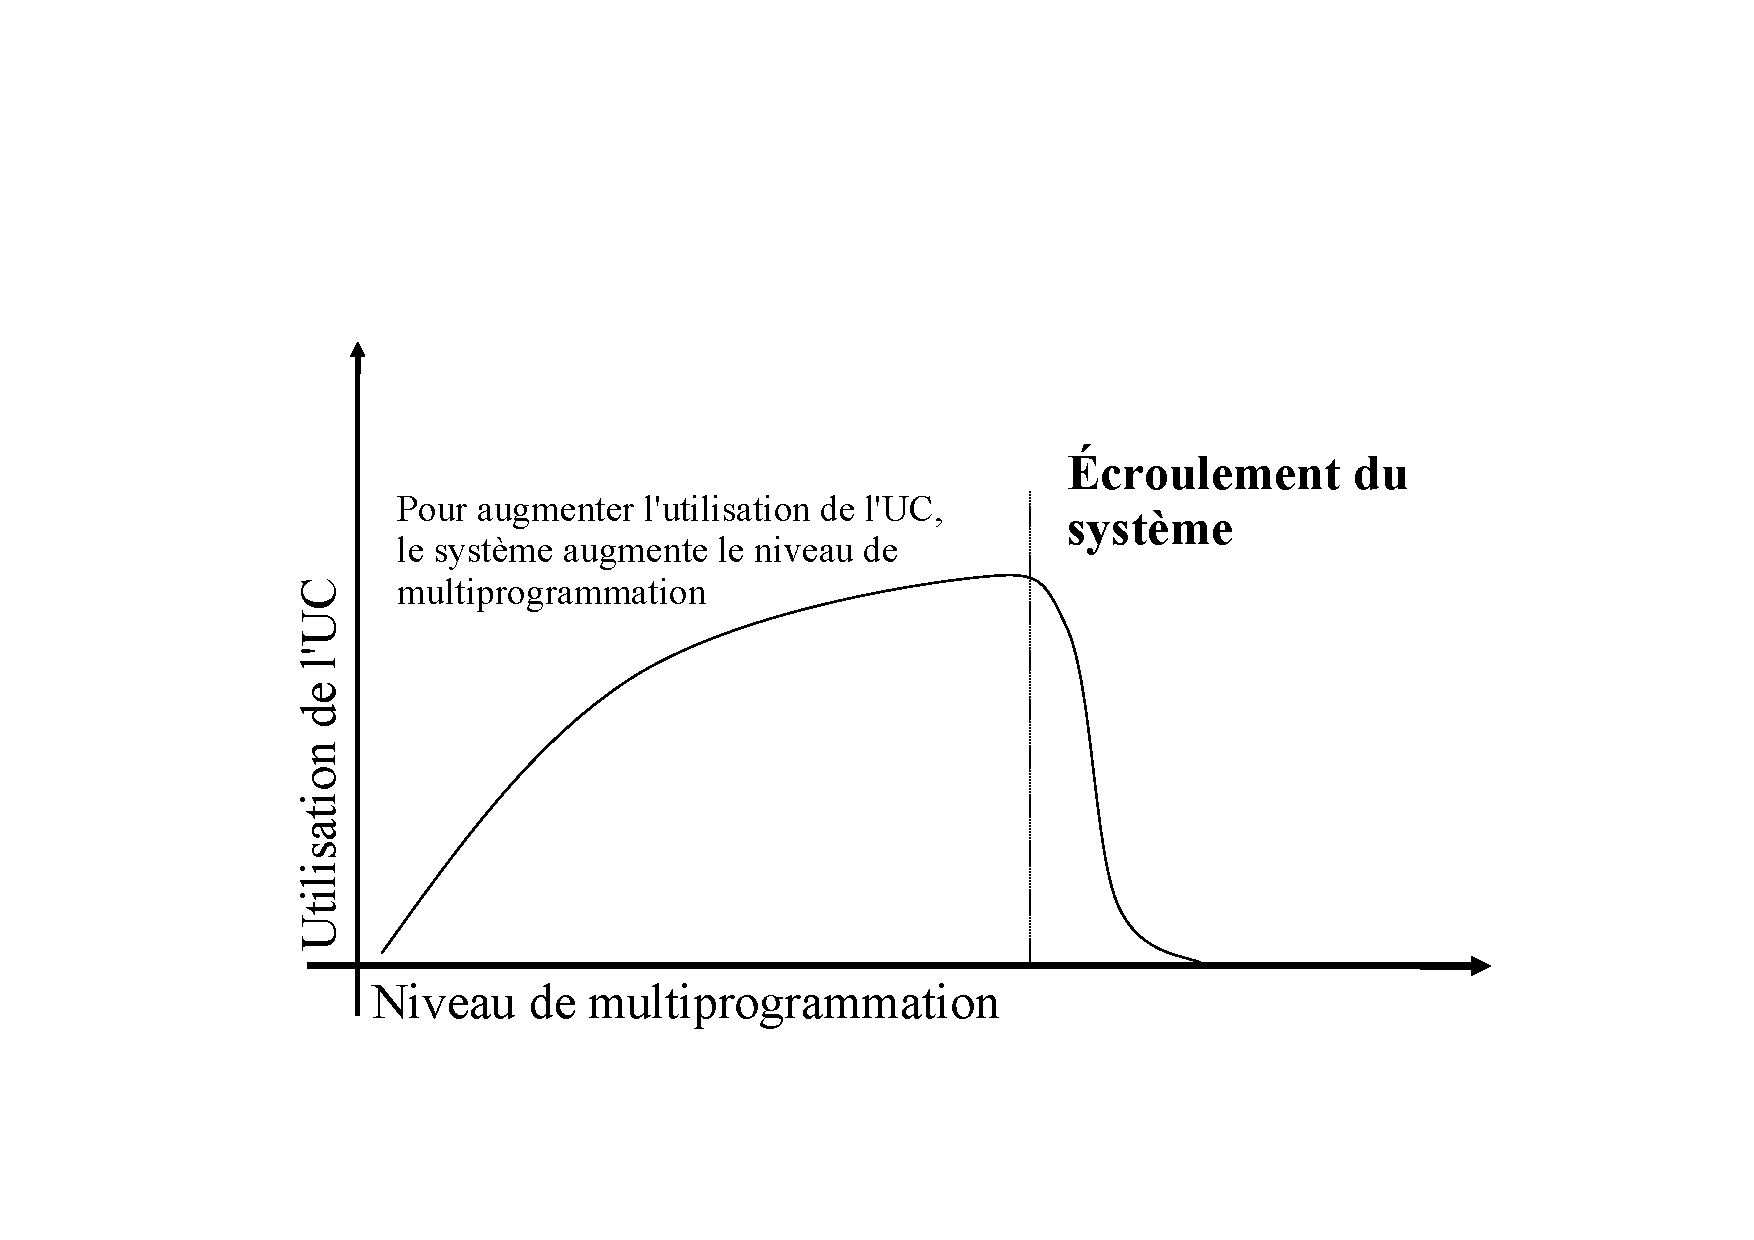
\includegraphics[width=.8\textwidth]{../illustration/Ecroulement.pdf}
\end{frame}

\begin{frame}
\frametitle{Solutions prventives / curatives  l'croulement du systme}
\begin{itemize}
\item Diminuer le niveau de multiprogrammation
\item Utiliser un algorithme de remplacement local ou prioritaire
\begin{itemize}
\item croulement local (limit  un processus)
\item Pour les autres : simple augmentation du temps de traitement des dfauts de page
\end{itemize}
\end{itemize}
\end{frame}


\begin{frame}
\frametitle{Solutions prventives / curatives  l'croulement du systme}
\begin{itemize}
\item Utiliser un modle de localisation de l'excution du processus
\begin{itemize}
\item Groupe de pages utilises ensemble
\item Principe de localit d'excution
\end{itemize}
\item Surveiller le taux de dfaut de page
\begin{itemize}
\item Maintenir le taux de dfaut de page dans une plage prdfinie
\end{itemize}
\end{itemize}
\end{frame}


\begin{frame}
\frametitle{Modle de l'ensemble de travail}
\begin{itemize}
\item Repose sur le principe de localisation
\begin{itemize}
\item Un processus utilise principalement une petite partie de son espace mmoire
\item Fentre de l'ensemble de travail
\end{itemize}
\item Observation de l'utilisation des pages
\begin{itemize}
\item Recherche les plus petits ensemble de travail
\item Chargement de l'ensemble de travail entier
\item Suspension si impossibilité de charger l'ensemble de travail en mémoire
\end{itemize}
\end{itemize}
\end{frame}


\begin{frame}
\frametitle{Recherche des ensembles de travail}
\begin{itemize}
\item Ensemble de travail
\begin{itemize}
\item Approximation de la localisation du processus
\item Utilisation active des pages
\end{itemize}
\item Observation des n dernires rfrences mmoire
\item Une page fait partie de l'ensemble de travail si elle est utilise au moins une fois au cours des n derniers cycles
\end{itemize}
\end{frame}


\begin{frame}
\frametitle{Exemple d'ensemble de travail}
\begin{itemize}
\item n = 10
\item Recherche de l'ensemble de travail W
\item Table de rfrence de page :
\end{itemize}
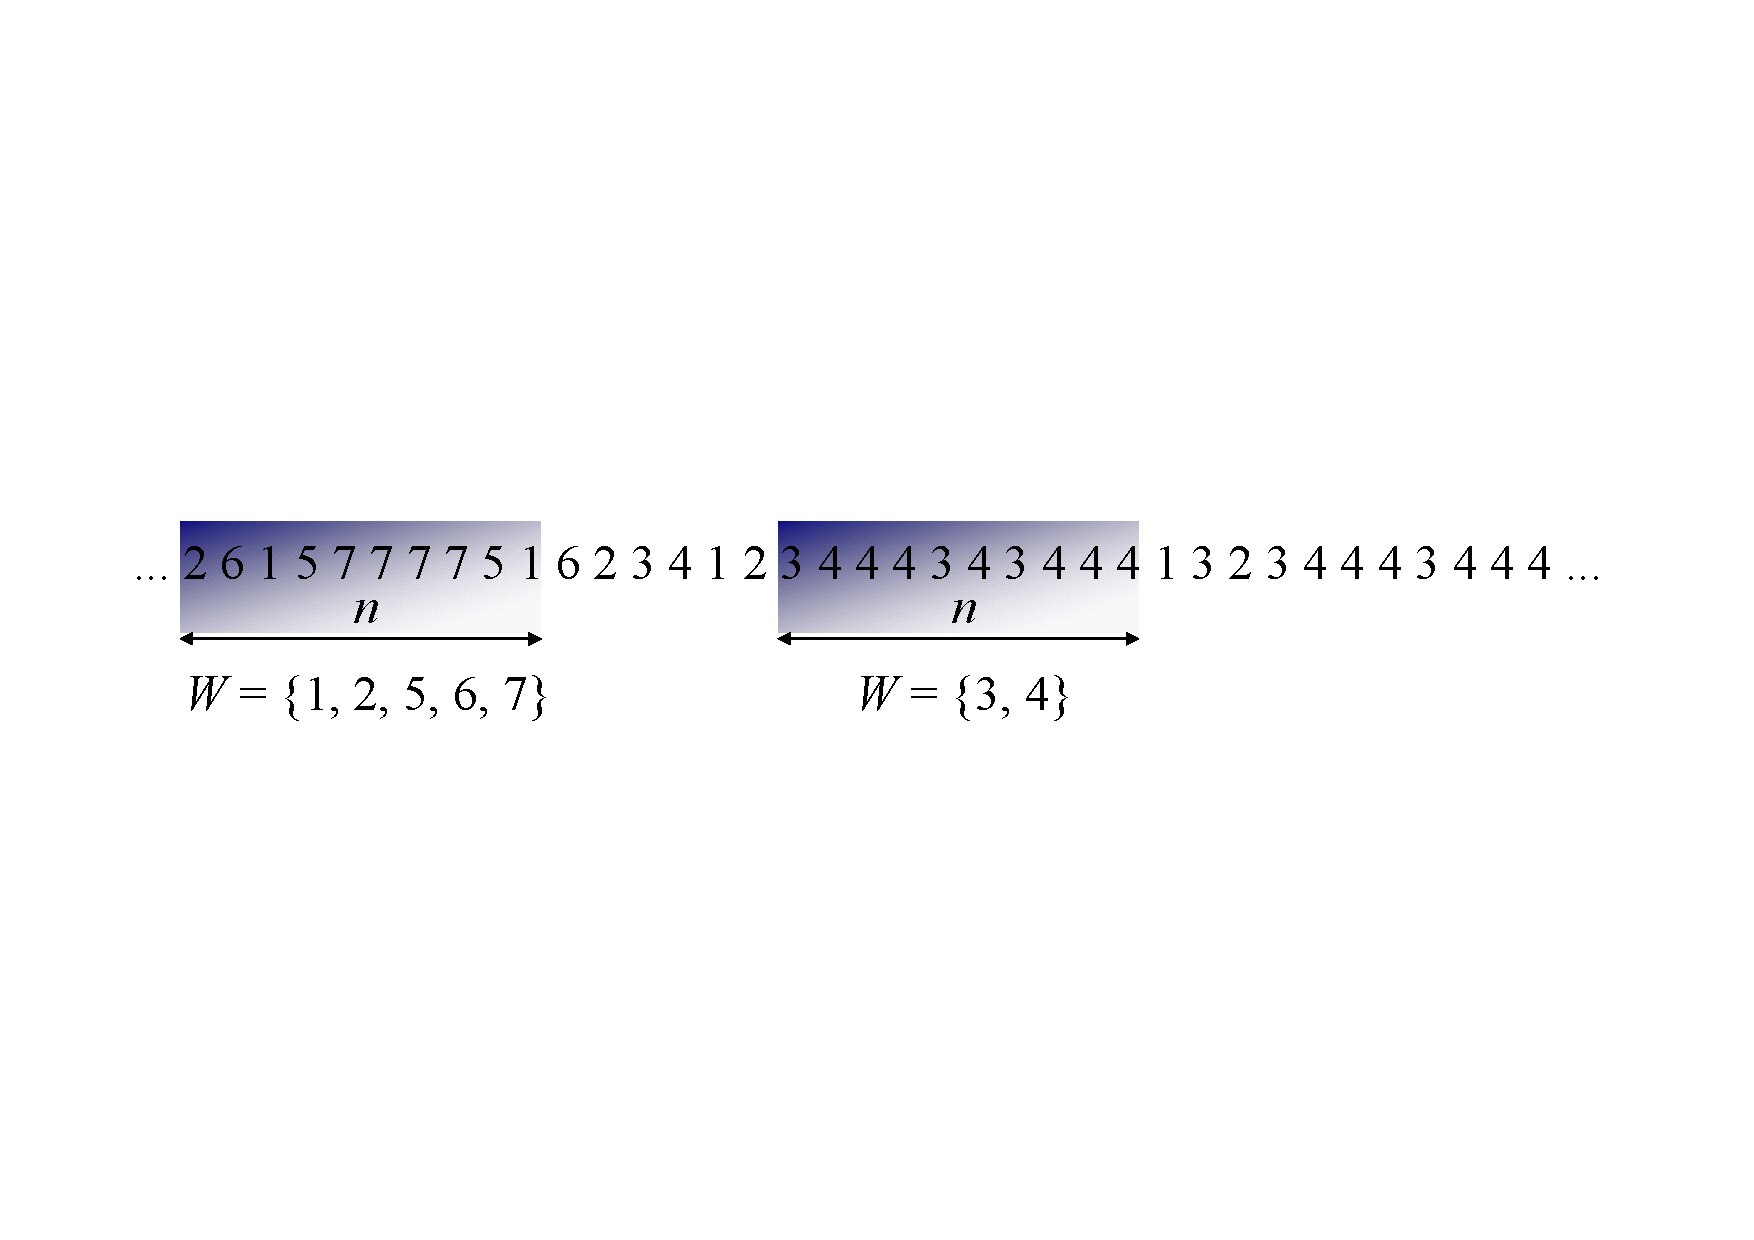
\includegraphics[width=.8\textwidth]{../illustration/ensemble_travail.pdf}
\end{frame}


\begin{frame}
\frametitle{Modle de l'ensemble de travail}
\begin{itemize}
\item Risque d'croulement si la somme des ensembles de travail des processus actifs est suprieure  la mmoire disponible
\item Aucun risque dans le cas contraire
\item Solution :
\begin{itemize}
\item Surveiller les ensembles de travail
\item Suspendre des processus lorsque la mmoire ne peut contenir tous les ensembles de travail
\end{itemize}
\end{itemize}
\end{frame}


\begin{frame}
\frametitle{Modle de l'ensemble de travail}
\begin{itemize}
\item Difficults :
\begin{itemize}
\item Surveillance continue du systme
\item Dfinition des ensembles mouvante
\end{itemize}
\item Algorithme performant en pratique
\begin{itemize}
\item Empche l'croulement
\item Maintient un niveau de multiprogrammation lev
\item Surcot de traitement des dfauts de page
\end{itemize}
\end{itemize}
\end{frame}



\begin{frame}
\frametitle{Taux de dfaut de page}
\begin{itemize}
\item Stratgie PFF 
\begin{itemize}
\item Frquence de dfaut de page
\end{itemize}
\item Dfinition de seuils haut et bas sur la frquence de dfaut de page
\begin{itemize}
\item Trop lev :
\begin{itemize}
\item Le processus a besoin de plus de page
\end{itemize}
\item Trop faible :
\begin{itemize}
\item Le processus peut librer des pages
\end{itemize}
\item Suspension de processus au besoin
\end{itemize}
\end{frame}


\begin{frame}
\frametitle{Stratgie PFF}
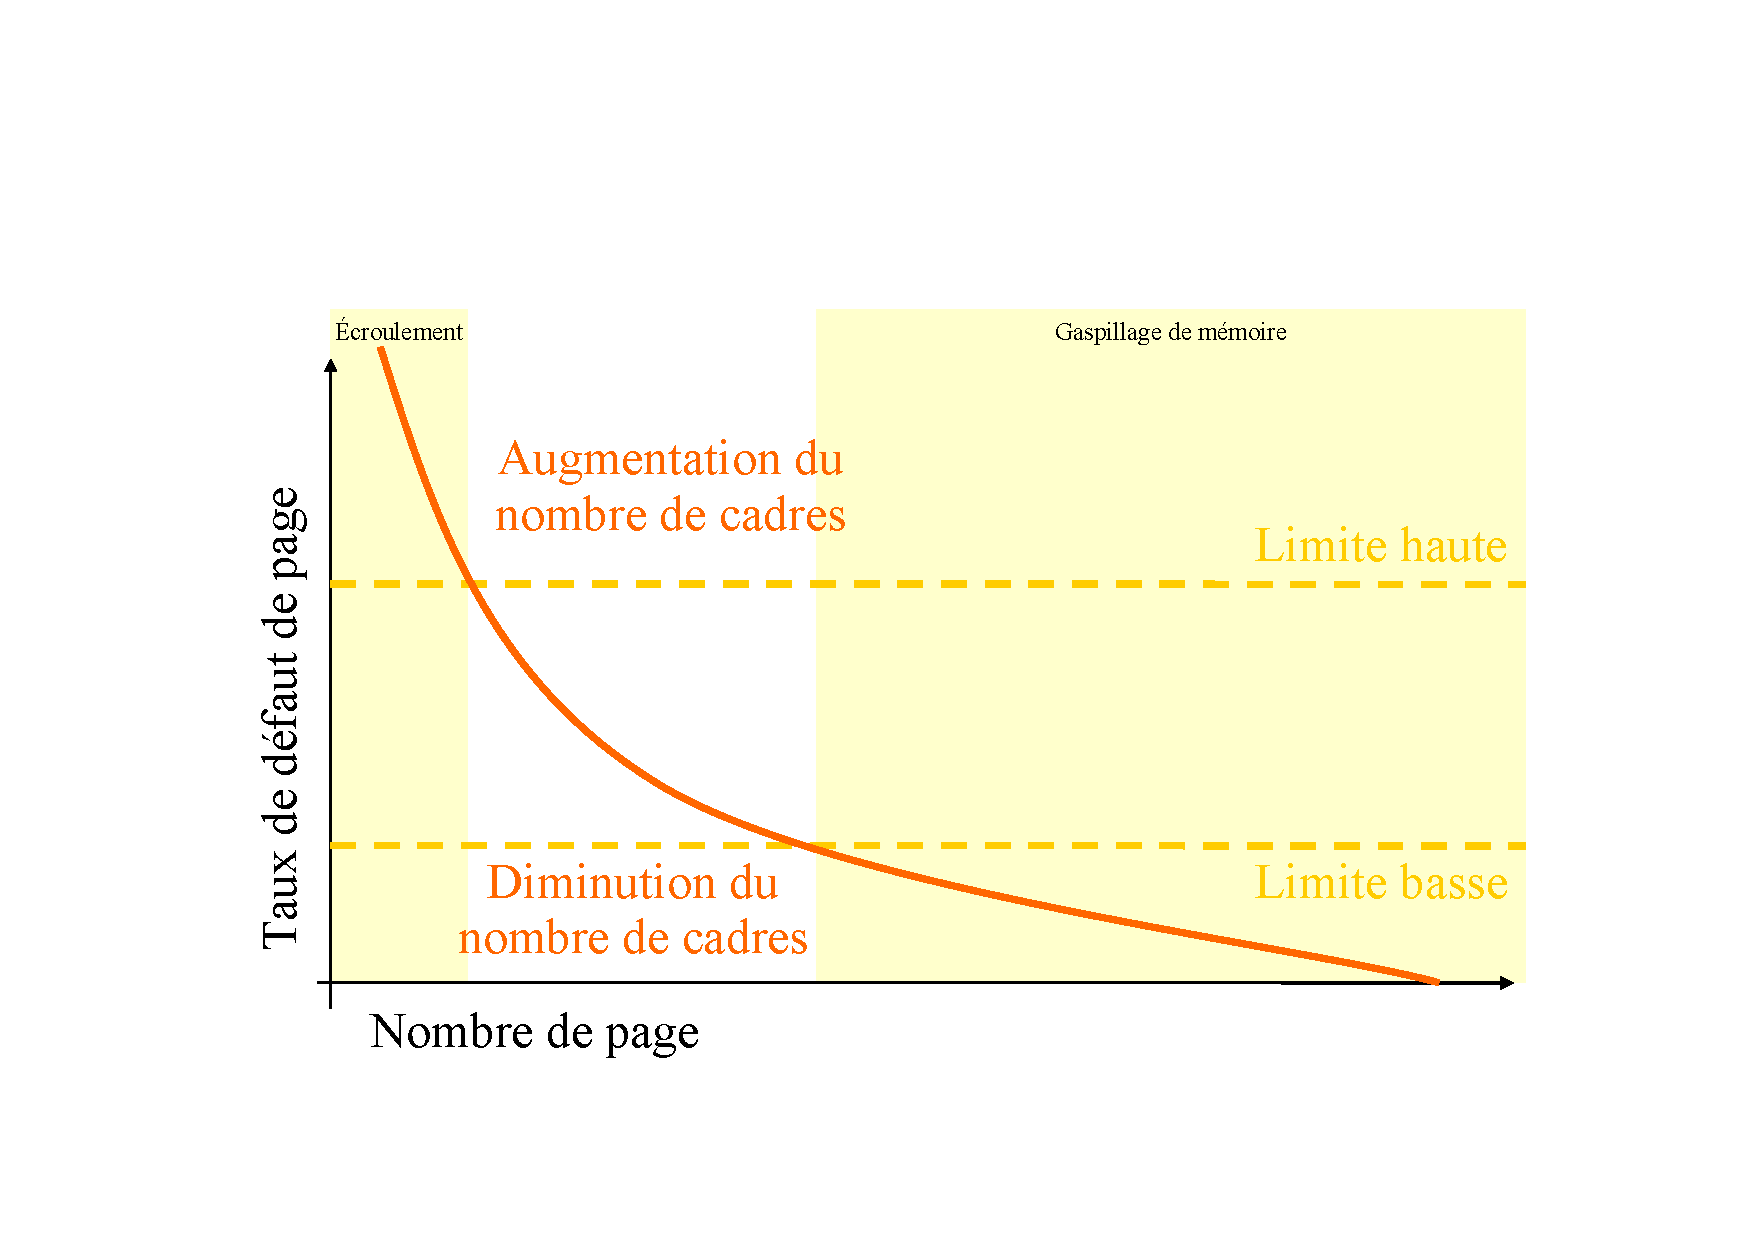
\includegraphics[width=.8\textwidth]{../illustration/Strategie_PFF.pdf}
\end{frame}


\begin{frame}
\frametitle{Algorithme d'allocation}
\begin{itemize}
\item Disque :
\begin{itemize}
\item Élément le plus lent d'un ordinateur
\item Principal goulot d'étranglement pour les performances du système
\item Limiter au maximum les accès au disque
\end{itemize}
\item Importance des algorithmes d'allocation
\item Exemple : Unix
\begin{itemize}
\item Maintient des données proches de l'inode
\item Allocation à l'avance des inodes
\end{itemize}
\end{itemize}
\end{frame}

\begin{frame}
\frametitle{Utilisation de caches}
\begin{itemize}
\item Sur le contrôleur de disque
\item En mémoire principale
\begin{itemize}
\item Partie réservée (cache disque)
\item Toute la mémoire disponible
\end{itemize}
\item Accès séquentiel :
\begin{itemize}
\item Lecture par anticipation
\item Libération arrière
\end{itemize}
\end{itemize}
\end{frame}


\frame[allowframebreaks]
{
\frametitle{Bibliographie}
\bibliographystyle{plain}
\bibliography{smb137}
}

\end{document}
